\begin{question}
  \hspace*{\fill} [Note Maximale: 6]\par
  \medskip
  \begin{center} % or flushleft or flushright
    \noindent La figure ci-dessous donne la représentation graphique d'une fonction $f(x)$ pour $ -2 \le x \le 3$.\par
    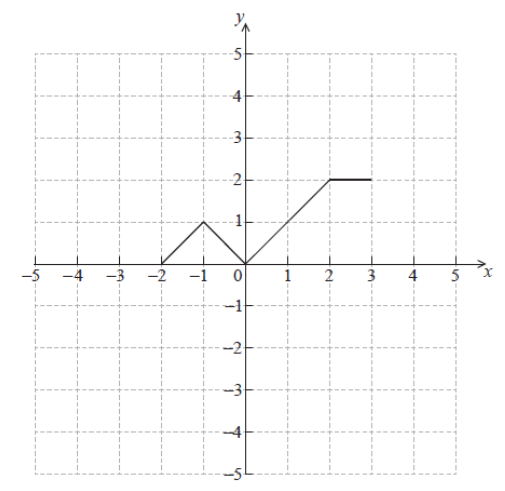
\includegraphics[scale=0.3]{diagramme_x4a}\par
    \noindent diagramme A\par
  \end{center} % or flushleft or flushright
  \begin{center} % or flushleft or flushright
    \noindent Système d'axe pour la réponse a)\par
    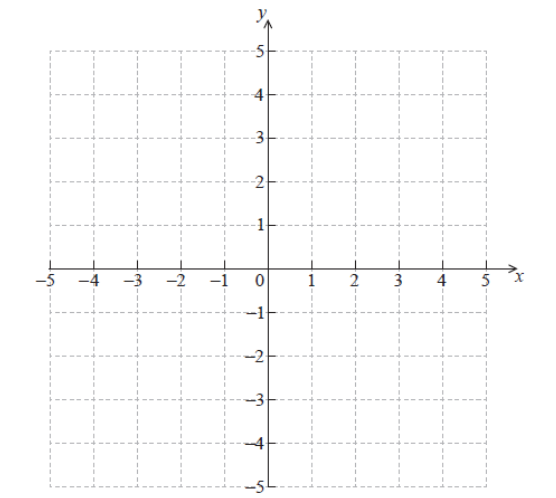
\includegraphics[scale=0.3]{diagramme_x4b}\par
    \noindent diagramme B\par
  \end{center} % or flushleft or flushright
  \begin{center} % or flushleft or flushright
    \noindent La représentation graphique de $f$ est transformée pour obtenir la représentation graphique de $g$. La courbe de $g$ est représentée ci-dessous \par
    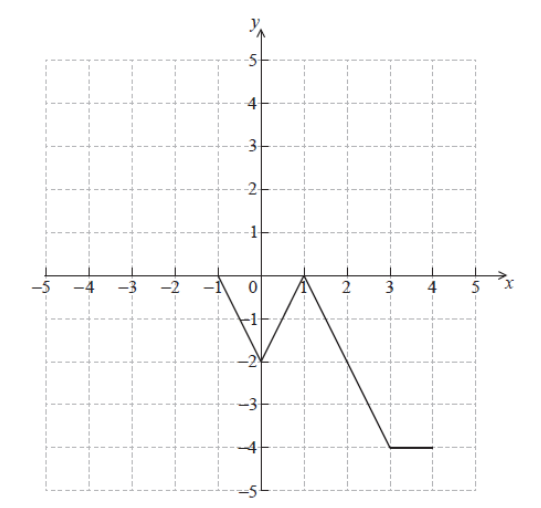
\includegraphics[scale=0.3]{diagramme_x4c}\par
    \noindent diagramme C\par
  \end{center} % or flushleft or flushright

  \begin{enumerate}[label=(\alph*)]
    \item Esquissez la representation graphique $f(-x)$ sur le système d'axe du diagramme B.\hspace*{\fill} [2]
    \item La fonction $g$  peut s'écrire sous la forme $g(x) = a\,f(x + b)$. Donnez la valeur de $a$ et celle de $b$\hspace*{\fill} [4]
  \end{enumerate}
\end{question}
